In program $p$, calling function $f$ with arguments $\vec{a}$\\
from initial memory $m$ terminates in final memory $m'$
and returns values $\vec{r}$:\\
[0.2cm]
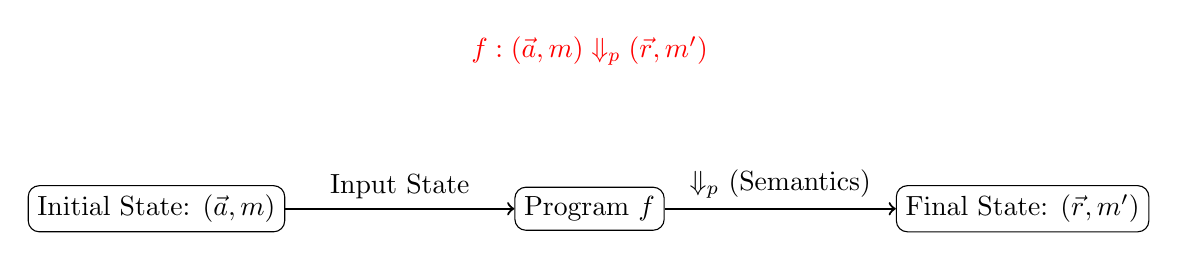
\begin{tikzpicture}[node distance=1.5cm, auto]
	% Nodes
	\node[draw, rectangle, rounded corners] (initial) {Initial State: $(\vec{a}, m)$};
	\node[draw, rectangle, rounded corners, right of=initial, xshift=4cm] (program) {Program $f$};
	\node[draw, rectangle, rounded corners, right of=program, xshift=4cm] (final) {Final State: $(\vec{r}, m')$};
	
	% Arrows
	\draw[->, thick] (initial) -- (program) node[midway, above] {Input State};
	\draw[->, thick] (program) -- (final) node[midway, above] {$\Downarrow_p$ (Semantics)};
	
	% Labels
	\node[above of=program, yshift=.5cm, align=center] {\color{red} $\boxed{f: (\vec{a}, m) \Downarrow_p (\vec{r}, m')}$};
\end{tikzpicture}
%\begin{enumerate}
%	\item Initial State (\( \vec{a}, m \)): Represents the input argument (\( \vec{a} \)) and the initial memory (\( m \)).
%	\item Program (\( f \)): The function or program being executed, transforming the state.
%	\item Final State (\( \vec{r}, m' \)): The output result (\( \vec{r} \)) and the updated memory (\( m' \)).
%	\item Execution Semantics (\( \Downarrow_p \)): Denotes the specific rules or semantics under which the program executes, determining how the transition happens
%\end{enumerate}
\\ [.5cm]
\begin{itemize}
	\item This is the definition of the program behaviors (formalized in Coq).
	\item All proofs are made relative to this definition.
\end{itemize}